\chapter{Planning}

%TODO: Add normal Definition here
\begin{definition} Markov decision process is formalized as a tuple $<S, A, P, R>$, where
\begin{itemize}{}
\item $S$ is a finite set of states of the environment.
\item $A$ is a finite of actions.
\item The transition function $P:S \times A \times S \rightarrow [0, 1]$ defines a probability distribution over the possible next states. 
\item The reward function $R:S \times A \rightarrow \mathbb{R}$ defines the reward after executing a certain action at a certain state.
\end{itemize}
\end{definition}

Given a state of the environment, a policy $\pi: S \times A)$ tells what action should be performed. 
The value function $V^{\pi}: S \times \mathbb{R}$ is the expected cumulative reward when executing
policy $\pi$ from state $s$.

The value function satisfies the Bellman equation:
\begin{equation}
    V^{\pi}(s) = \sum_{s'}P(s'|s, \pi(s))[R(s, \pi(s)) + \gamma V^{\pi}(s')],
\end{equation}
where $\gamma \cin [0, 1]$ is the discount factor which discounts the future reward to the present value.

Similarly, we define the action-value function (or Q function) as:
\begin{equation}
    Q^{\pi}(s, a) = \sum_{s'}P(s'|s, \pi(s))[R(s, \pi(s)) + \gamma Q^{\pi}(s', \pi(s'))].
\end{equation}
The Q function is the expected cumulative reward after executing action $a$ at state $s$ and following
$\pi$ thereafter.

Now lets us extends action set $A$ to include composite actions.

We also need to explicit model the time limit for a composite action to execute, since it
is possible for a composite action to have unachievable terminal state (why?). We do not want 
to wait for the composite action to infinity.

The transition function $P$ and $R$ are modified to include the time limit $t$:
\begin{equation}
    P(s'|s, a, t) = \sum^t_{k=1} \gamma^k Pr(k, s'|s, a),
    \ref{eq:multiProb}
\end{equation}
\begin{equation}
    R(s, a, t) = \sum^t_{k=0} \gamma^k r_k,
\end{equation}
The value function needs to be modified as:
\begin{equation}
    V^{\pi}(s) = \sum_{s'}P(s'|s, \pi(s), t)[R(s, \pi(s), t) + \gamma^N V^{\pi}(s')],
\end{equation}
where $N$ is the number of steps for the action $\pi(s)$ to finish its execution.
A question arises since we do not know the actual time to finish executing each composite action.
Let's set $gamma=1$ from now on.
%TODO: (how MaxQ solve it?).

Although the state abstraction provides us compact state representation, 
it doesn't change the size of the planning envelope. Thus we do not gain any computational
advantage by applying such an abstraction technique.

A key observation of this work is to adopt an unsafe projection function. 
The size of planning envelope grows exponentially with the number of features.
By assuming 
some features do not change during the execution of actions, we do gain computational advantage by
significantly reducing the size of the planning envelope. 
We lose the optimally with this approximation technique, but it is necessary because we want 
to apply our work beyond toy applications.
Our approach doesn't imply that
part of the features are completely ignored. The agent still computes the plan according to 
the new value of t)e features.
Besides, the model-free layer still operates with the full observation of the state. 
If we put more features into the model-based layer, we would get a more precise plan at the cost
of more samples required to estimate the model parameter and more time spent on computing the plan.
Therefore, the number of features included in the model-based layer depends on the available 
computation resources.
The objective of our work is not to show how to find the optimal arrangement of features, but to indicate
that there is a trade-off between model-based and model-free approaches.
By adjusting the arrangement of features, we can maximize the performance of the agent without exceeding
the capacity of available computational resources.
%TODO: the grid world example--> assuming monster does not move is correct
%TODO: show that approximation is necessary--> the planning envelope is exponentially huge wrt the number of monsters

To compensate the incapability to predict the movement of the monsters in the long run, 
we exploits the model-free approach to handle the dynamic of the environment in the short period.
The choice

\section{Estimation of the transition probability}

Each model-based layer (except the top one) needs to compute the state transition probability
from the given state $s$ to some terminal state $x$.
\begin{equation}
    P(x|s) = max_a P(x|s, a).
\end{equation}
\begin{equation}
    P(x|s, a) = P() from all other states
\end{equation}
It can be done by querying the transition probability from the child layers.
Same for the reward.

Each model-free layer with a parent model-based layer also needs to compute the transition probability.
Since the child layers of model-free layer do not provide such information, the model-free layer
needs to estimate the probability based on its current policy.

%1. Assumption on the state difference (if it is not true --> like the agent in a world boundary or the health is 100 and cannot be imporve
  %since the state is outside the known state boundary, the planner whon't plan for it. but the local planner may still direct the agent
  %to go outside the world boundary, which may be a problem)
%2. Application to the hierachical RL
%3. Limitation: unachievable state (a coin surrounded by many monsters)
%4. Can inference in a very small world, not need to do 64 by 64
%Sometimes we need a plan. The greedy approach of reinforcement learning does not always work. 
%RL techniques have several limitations:
%1. It's difficult for to transfer the value function from a small world to a large one. If the agent has
%the experience only in a small world like 4 \times 4 grid, it cannot act well in 64 \times 64 grid
%because it does not know the correct action in regard to an object 63 grid away.

%2. It takes a long time to train the agent to be good enough. The greedy 

%3. The approximation only good in a small range. We need a plan for long term action.
%The noval state (the state in current game which has not been experienced) may 

%4. Impossible task to maze problems: RL require that optimal agent to find the optimal solution for a maze when all the features
%are input to the agent. Which is unlikely to work.(impractical when the maze is large)(unable to transfer
%the knowledge from previous maze experience to the current one) A practical solver shall invovle planning through 
%the possible route and find the one which can lead to the exist.
%All the work requires the agent to repeat play the same maze (assuming traps) until it finds the optimal solution.
%What if the maze changes every time?

%1. Is it guarranteed convergence? Yes, if we choose the goal next to the current state which leads to highest Q value. 
%It is the same as SARSA.
%2. How to choose the goal to guarrante convergence to optimal policy?

%Good to work on the problem with a long term reinforcement (feedback) like a maze.
%Bad to work with a problem with dynamic envirment (everything changes with or without agents actions)
%Bad when the consequence of an action is delayed for many steps. (poison)

%Q: prove that RL cannot solve maze problem
%Ability to transfer the knowledge from one maze to another
%compare the HRL in key-finding problem
%compare to the model-based RL

%1. Example: Grid world u
\begin{figure}[h]
    \centering
    \begin{minipage}[t]{0.3\linewidth}
        \centering
        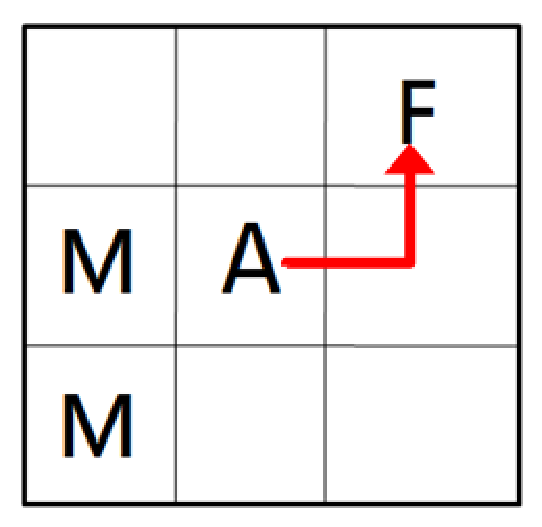
\includegraphics[width=\textwidth] {./figures/monster_plan.eps}
    \end{minipage}
    \caption{The shortest path from the agent's location to the food}
    \label{fig:monster_plan}
\end{figure}
Consider the eat-food-and-avoid-monster game in Fig. \ref{fig:monster_plan}. If the monsters do not move and the actions are deterministic
, the optimal policy of the game can be founded by the shortest path algorithm. The goal state is the location of the food,
the cost to move to the adjacent location is $1$, if there is a monster in the adjacent location, the cost 
to move to it is $\infty$. The agent only needs to compute the lowest cost path from its current position to the goal,
and choose the action which can keep it on this precomputed path.

However, the game is not a static one. The monsters may move around and block the precomputed path. The actions of
agent may have unpredictable result to lead it out of the precomputed path.
This stochastic natural of the game makes it natural to formulate the problem as a stochastic shortest path
problem. A stochastic shortest-path (SSP) problem is a MDP problem with a absorbing goal state and positive costs.
A solution of a SSP problem is a policy from the initial state to the goal state with minimum expected cost.

A work by Zucker et al. \cite{Planner} introduced a two-level approach to solve a maze problem.
The planner uses the shortest path algorithm to find a path from the current state to the goal state.
The cost of each step is estimated by Q value, which is computed by the SARSA algorithm.

A issue occurred when we want to apply this approach to general MDP problems: we do not know the 
goal state. The objective of MDP is to find a sequence of actions which can maximize the overall 
rewards. There are no clearly defined "goal" for the MDP problems.

A possible way to adopt the planning technique to the MDP problems is to choose a sequence 
of goals which can maximize the overall rewards. The goal can be chosen to be the state
with the highest expected reward. To achieve this, an agent needs to learn 
the probability to move from one state to another, and the reward to be received
from each state. 

The approach is two fold. In the beginning, the planner selects a path from the current 
state to the goal state with the highest expected reward. The path consists of several
nodes, which are considered as the subgoals of the plan. The RL agent finds the subgoal 
right after the current state, and chooses a sequence of actions which can lead the agent
to the subgoal. The result can be either success or failure, and the probability of the successful
rate of a plan would be updated accordingly. The planner then use the updated information to 
compute a new path.


%application: the key-room problem--> each room lock a key, one room has a treasure, the agent needs to go through 
%a maze to collect the keys for each door and get the treasure

%Stochastic Shortest-Path Problems
%A Stochastic Shortest-Path problem is an mdp prob-
%lem in which the state space S = f1; : : : ; n; tg is such
%that t is a goal (target) state that is absorbing (i.e.,
%p(t; u; t) = 1 and g(t; u) = 0 for all u 2 U(t)), and the
%discount factor ® = 1. In this case, the existence of
%optimal policies (and optimal stationary policies) is a
%major mathematical problem. However, the existence
%is guarantee under the following reasonable conditions:
%(A1) There exists a policy that achieves the goal with
%probability 1 from any starting state.
%(A2) All costs are positive.
%The ¯rst assumption just expresses the fact that the
%problem admits a well-behaved solution. Such policies
%are known as proper policies. The second assumption,
%in the other hand, guarantees that all improper policies
%incurs in in¯nite cost for at least one state. Thus, both
%assumptions preclude cases where the optimal solution
%might \wander" around without never getting to the
%goal. For example, a problem having a zero-cost cycle
%(in state space) violates the second assumption.
%As mentioned in the Introduction, often we are only
%interested in knowing how to go from a ¯xed initial
%state, say 1, to the goal state. The optimal solution in
%this case is an partial optimal stationary policy ¹ such
%that ¹(i) = ¹¤(i) for all states i that are reachable
%from 1 when using the optimal policy ¹¤; the so-called
%relevant states when starting from 1.1
%Finding a partial optimal policy can be consider-
%ably simpler, the extreme case when the set of relevant
%states is ¯nite and the complete state space is in¯nite.
%Thus, the question of how to ¯nd partial optimal poli-
%cies is of great relevance. One algorithm for that is
%Real-Time Dynamic Programming.

